%%%%%%%%%%%%%%%%%%%%%%%%%%%%%%%%%%%%%%%%%%%%%%%%%%%%%%%%%%%%%%%%%%%%%%%%%%%%%%%%
%%
%% Para utilizar ese modelo sao necessarios os seguintes arquivos:
%%
%% copin.cls
%% copin.sty
%% mestre.sty
%%
%%%%%%%%%%%%%%%%%%%%%%%%%%%%%%%%%%%%%%%%%%%%%%%%%%%%%%%%%%%%%%%%%%%%%%%%%%%%%%%%

\documentclass[a4paper,titlepage]{copin}
\usepackage[utf8]{inputenc}
\usepackage[T1]{fontenc}
\usepackage[brazilian,english]{babel}
\usepackage{copin,mestre,epsfig}
\usepackage{times}

%-------------------------- Para usar acentuacaoo em sistemas ISO8859-1 ------------------------------------
% Se estiver usando o Microsoft Windows ou linux com essa codificacao, descomente essa linhas abaixo
% e comente as linhas referentes ao UTF8
% \usepackage[latin1]{inputenc} % Usar acentuacao em sistemas ISO8859-1, comentar a linha com  \usepackage[utf8x]{inputenc}
%-----------------------------------------------------------------------------------------------------

%-------------------------- Para usar acentuacao em sistemas UTF8 ------------------------------------
% Para a maior parte das distribuicoes linux, usar a opcao utf8x (lembrar de comentar as linha referente a ISO8859-1 acima)
\usepackage{ucs}
%\usepackage[utf8x]{inputenc}
%\usepackage[utf8]{inputenc}
% \usepackage[T1]{fontenc}
%-----------------------------------------------------------------------------------------------------


\usepackage{fancyheadings}
\usepackage{graphicx}
\usepackage{longtable} %tabelas longas, para tabelas que ultrapassam uma pagina
%\input{psfig.sty}


% ----------------- Para inserir codigo fonte de linguagens de programacao no documento -------------
\usepackage{listings}
\lstset{numbers=left,
stepnumber=1,
firstnumber=1,
%numberstyle=\tiny,
extendedchars=true,
breaklines=true,
frame=tb,
basicstyle=\footnotesize,
stringstyle=\ttfamily,
showstringspaces=false
}
\renewcommand{\lstlistingname}{Código Fonte}
\renewcommand{\lstlistlistingname}{Lista de Códigos Fonte}
% ---------------------------------------------------------------------------------------------------

\selectlanguage{brazilian}
\sloppy



\begin{document}



%%%%%%%%%%%%%%%%%%%%%%%%%%%%%%%%%%%%%%%%%%%%%%%%%%%%%%%%%%%%%%%%%%%%%%%%%%%%%%%%
\Titulo{Explorando o Compartilhamento de Conteúdo em Redes Sociais para Fomentar Sites \\de Perguntas e Respostas }
\Autor{Lenin da Nóbrega Medeiros}
\Data{19/06/2015}
\Area{Ciência da Computação}
\Pesquisa{Sistemas de Computação}
\Orientadores{Dr. Nazareno Ferreira de Andrade  \\
	 (Orientador)}

\newpage
\cleardoublepage

\PaginadeRosto

\newpage
\cleardoublepage

%%%%%%%%%%%%%%%%%%%%%%%%%%%%%%%%%%%%%%%%%%%%%%%%%%%%%%%%%%%%%%%%%%%%%%%%%%%%%%%%
\begin{resumo} 
Sites \qa são aqueles acessados por usuários com o intuito de: encontrar uma resposta para alguma pergunta ou ajudar alguém a conseguir isto. Tais sites são muito utilizados, por exemplo, por programadores que desejam esclarecer dúvidas gerais sobre programação, como é o caso do site \textit{Stack Overflow em Português}. Muitos pesquisadores têm concentrado esforços visando descobrir maneiras de atrair mais conteúdo para sites deste tipo e, também, entender comportamentos e motivações dos respectivos usuários. Investigou-se, neste trabalho, a utilização da prática do compartilhamento de perguntas oriundas de sites \qa em redes sociais como estratégia para fomentar a contribuição em tais sites. Nosso intuito era: entender como os usuários se comportam diante de tal funcionalidade, investigar como promover tal prática e, por fim, tentar encontrar indícios acerca da utilidade desta prática como meio de fomentar a contribuição em sites \qanospace. Foram feitas duas investigações qualitativas nas quais usuários de sites \qa e de redes sociais foram entrevistados e relataram como se comportam diante do compartilhamento de perguntas. Posteriormente, foi realizado um experimento quantitativo para testar diferentes formas de incentivar o compartilhamento de perguntas oriundas de sites \qa em redes sociais, bem como para investigar mais a fundo o efeito desta prática no conteúdo destes sites. Descobriu-se que os usuários são muito criteriosos na escolha dos conteúdos que eles compartilham nas suas redes sociais por causa dos custos sociais envolvidos. Por este motivo concluímos que é preciso repensar a forma com a qual se tenta promover o compartilhamento de perguntas de tais sites em redes sociais. Além disto, também foi possível perceber que tal compartilhamento pode não ser uma boa escolha para quem pretende fomentar a contribuição nestes sites em questão.
\end{resumo}

\newpage
\cleardoublepage

%%%%%%%%%%%%%%%%%%%%%%%%%%%%%%%%%%%%%%%%%%%%%%%%%%%%%%%%%%%%%%%%%%%%%%%%%%%%%%%%
\begin{summary}
\qa sites are those which are accessed by users who want to find some answer to some question or help someone else to get this. These websites are very used, for instance, by programmers in order to clarify general questions about programming. This behavior could be found in a website called \textit{Stack Overflow em Português}. Many researchers have been focused on finding out ways to attract more content to these websites and, also, on the aspects of behaviors and motivations of its users. In this work our focus was the use of the practice of sharing \qa sites questions in social networks as strategy to increase the content of these websites. Our aim was: to extract some lessons about how is the users' behavior when they face the functionality of to share questions in \qa sites, investigate how to promote this behavior and find out evidences about the advantages for \qa sites related to this practice as way to increase the contribution to this kind of websites. We conducted two qualitative investigations in which users from \qa sites and social networks were interviewed and they related how were they behaviors when they faced the sharing of questions. Then, we made a quantitative experiment in order to test different ways of promoting the sharing of \qa sites questions in social networks, as well as to investigate more deeply the effect of this practice in these websites contents. We found that the users are very discerning when they decide to share or not content in their social networks because of the related social costs. That's why we believe that it's necessary to change the way to promote the sharing of \qa sites questions in social networks. Besides that, it's also possible to notice that this sharing of questions may not be a good strategy to increase the contribution in these websites.  
\end{summary}

\newpage
\cleardoublepage

%%%%%%%%%%%%%%%%%%%%%%%%%%%%%%%%%%%%%%%%%%%%%%%%%%%%%%%%%%%%%%%%%%%%%%%%%%%%%%%%
\begin{agradecimentos}
Agradeço a Deus, sempre, a saúde e as oportunidades que a mim foram dadas. Agradeço aos meus pais, seu Glauco e dona Terezinha, o apoio incondicional e o zelo com o qual a minha educação básica foi tratada desde quando eu nasci. Agradeço aos demais membros da minha família que também me apoiaram, de alguma forma, durante esta minha empreitada.

Agradeço aos amigos do grupo \textit{OFF Thread} a sincera e carinhosa amizade.

Agradeço ao meu orientador, o professor Nazareno Andrade, os valiosos ensinamentos que levarei comigo durante toda a minha jornada profissional.

Agradeço a todos aqueles que participaram das minhas investigações, tanto por meio das entrevistas concedidas quanto por meio da utilização do site \textit{Dê uma Força para o Stack Overflow em Português!}

Agradeço aos professores e colegas pesquisadores do \textit{LSD}, especialmente: Felipe Vieira, Nigini Abilio, Lesandro Ponciano, Milena Araujo e Aline Morais.

Agradeço ao governo brasileiro que, por meio da Coordenação de Aperfeiçoamento de Pessoal de Nível Superior, financiou a minha pesquisa de mestrado durante o último biênio.
\end{agradecimentos}

\clearpage

%%%%%%%%%%%%%%%%%%%%%%%%%%%%%%%%%%%%%%%%%%%%%%%%%%%%%%%%%%%%%%%%%%%%%%%%%%%%%%%%
%% Definicao do cabecalho: secao do lado esquerdo e numero da pagina do lado direito
\pagestyle{fancy}
\addtolength{\headwidth}{\marginparsep}\addtolength{\headwidth}{\marginparwidth}\headwidth = \textwidth
\renewcommand{\chaptermark}[1]{\markboth{#1}{}}
\renewcommand{\sectionmark}[1]{\markright{\thesection\ #1}}\lhead[\fancyplain{}{\bfseries\thepage}]%
	     {\fancyplain{}{\emph{\rightmark}}}\rhead[\fancyplain{}{\bfseries\leftmark}]%
             {\fancyplain{}{\bfseries\thepage}}\cfoot{}

%%%%%%%%%%%%%%%%%%%%%%%%%%%%%%%%%%%%%%%%%%%%%%%%%%%%%%%%%%%%%%%%%%%%%%%%%%%%%%%%
\selectlanguage{brazilian}

\Sumario
\ListadeSimbolos
\listoffigures
\listoftables
\lstlistoflistings %lista de codigos fonte - Para inserir a listagem de codigos fonte
\newpage
\cleardoublepage

\Introducao


%%%%%%%%%%%%%%%%%%%%%%%%%%%%%%%%%%%%%%%%%%%%%%%%%%%%%%%%%%%%%%%%%%%%%%%%%%%%%%%%
%
% Hifenizacao - Colocar lista de palavras que nao devem ser separadas e que 
% nao estao no dicionario portugues.
% As palavras do dicionario portugues ja sao separadas corretamente pelo lateX
%
\hyphenation{ Hardware Software etc  }


%%%%%%%%%%%%%%%%%%%%%%%%%%%%%%%%%%%%%%%%%%%%%%%%%%%%%%%%%%%%%%%%%%%%%%%%%%%%%%%%
%% A partir daqui coloque seus capitulos. Sugere-se que eles sejam inseridos com o comando \input
%% Da seguinte maneira:
%%
%% \chapter{Introdução}

\section{Seçãoo 1 do Capítulo 1}
\subsection{Subseção}
\subsubsection{Subsubseção}

A Figura \ref{fig:sistemaProposto}. A Tabela \ref{tab:tabelaTeste}. A Equação (\ref{eq1}). O trabalho de fulano~\cite{ref1}. O Código Fonte \ref{cod1}.

\begin{figure}[htbp]	
\begin{center}
		\fbox{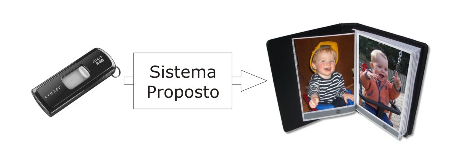
\includegraphics[scale=1]{sistemaProposto.eps}}
	\end{center}
	\caption{Sistema proposto}
	\label{fig:sistemaProposto}
\end{figure}

\begin{table}[htpb]
\begin{center}
\begin{tabular}{|c|c|c|}
\hline
coluna 1 & coluna 2 & coluna 3 \\
\hline
valor 1,1 & valor 1,2 & valor 1,3 \\
valor 2,1 & valor 2,2 & valor 2,3 \\
\hline
\end{tabular}
\end{center}
\caption{Primeira tabela.}
\label{tab:tabelaTeste}
\end{table}

\begin{equation}
E = m \times c^2
\label{eq1}
\end{equation}

\begin{lstlisting}[caption={Loop simples},label=cod1,numbers=none]
for(int x=1; x<10; x++){
  cout << x << "\n";
}
\end{lstlisting}

\section{Seção 2 do Capítulo 1}  
\subsection{Subseção}
\subsubsection{Subsubseção}

 
%% \input{cap2}
\chapter{Introdução}
    \begin{itemize}
        \item LEMBRAR DE DEFINIR O QUE SÃO REDES SOCIAIS AQUI NA INTRODUÇÃO;
        \item O que são sites de Q\&A. Exemplificar.
        \item Um Site que se sobresai é o SO. Exibir números para enfatizar a grandeza e importância do \textit{Stack Overflow}: quantidade de usuários, volume de conteúdo gerado, tempo médio de obtenção de resposta para as perguntas feitas no site, etc.; 
        % O site \textit{Stack Overflow}\footnote{http://stackoverflow.com/} é um exemplo do tipo destacado acima. Tal ambiente colaborativo foi concebido em 2008 e é creditado como o maior site de perguntas e respostas voltados para programadores que desejam tirar dúvidas e oferecer ajuda [REF]. Possui aproximadamente dois milhões de contribuidores [REF] e costuma ter suas perguntas respondidas em um tempo mediano de 11 minutos [REF].

% Em 2014, foi criada uma versão em português do site supracitado chamada \textit{Stack Overflow em Português}, com pouco mais de 14 mil usuários registrados [REF]. Tal site foi utilizado como estudo de caso nesta pesquisa (isto está exposto em detalhes mais adiante nesta dissertação).
        \item Promover contribuições é uma parte fundamental de operar sites deste tipo.0
        \item Visão geral de como tais sites estão estudados na literatura quanto a formentar contribuições;
        \item A motivação deste estudo parte de uma experiência prática com a operação de um site de QA,
        \item Descrever Forrósquare aqui, mencionar que esbarramos em dificuldades de fomentar o uso do sistema, e que percebemos a oportunidade de usar redes sociais já estabelecidas como forma de alimentar o site. (Nao alongar essa parte. Ela serve para inspirar a ideia de usar outras redes, e depois ligamos dizendo que voltando para a literatura, não encontramos estudos sobre isso).
            \begin{itemize}
                \item O que era o projeto Forrósquare?
                \item Quando, onde e como aconteceu?
                \item Qual era o intuito?
                \item O que se descobriu com os dados gerados pelo Forrósquare?
                \item Explicar que, graças ao Forrósquare, os pesquisadores se perguntaram a relação entre compartilhamento de perguntas em redes sociais e os sites \textit{Q\&A} (explicar como se chegou a tal questionamento);
                \item Redes sociais podem ser descritas como serviços da web nos quais é permitido a um dado usuário: criar um perfil público ou semi-público dentro de algum escopo limitado, articular alguma lista contendo outros usuários do mesmo serviço com os quais ele possui algum tipo de conexão e, ainda, visualizar e percorrer esta lista de conexões, bem como as listas de conexões dos outros usuários \cite{ellison2007social}. O objeto de estudo deste trabalho é um site \qa que não se comporta como uma rede social, tendo em vista que não atende aos 3 requisitos listados anteriormente. Vale ressaltar que é possível que algum site desta natureza também seja uma rede social. 
            \end{itemize}
        \item Explicar, resumidamente, o que foi feito a partir do Forrósquare e os resultados obtidos:
            \begin{itemize}
                \item Entendi como funciona o compartilhamento de perguntas de sites \textit{Q\&A} do ponto de vista dos usuários;
                \item Vi o que os dados quantitativos reais do Stack Overflow me disseram sobre a questão do compartilhamento;
                \item A partir do estudo qualitativo, defini 3 propostas de \textit{design} e vi como os usuários se comportaram em relação a elas por meio do umaforcaso.pt;
                \item Vi o que os dados quantitativos reais do umaforcaso.pt me disseram sobre a questão do compartilhamento;
                \item Minhas conclusões gerais do trabalho.
            \end{itemize}
\end{itemize}

\section{Motivação}

DO ARTIGO SOBRE O ESTADO DA ARTE DE SQA: It is becoming less and less accurate to think of SQA sites in a vacuum. Social networking sites such as Facebook allow the sharing of questions users find interesting on any SQA site, and it is possible to rate and interact with the same SQA content across multiple platforms.

    Discutir aqui a motivação deste trabalho:
    \begin{itemize}
        \item Investigar o que pode trazer mais conteúdo satisfatório (resposta para perguntas) é algo bem presente na literatura. Então, sempre existe demanda para investigar novas maneiras de fazer isto. Aqui eu vou investigar se o compartilhamento de perguntas pode ajudar, neste sentido, o Stack Overflow. Sendo assim, esta é uma motivação;
        \item Mostrar que as redes sociais estão bastante presentes na Internet e praticamente todos os sites possuem algum tipo de integração com elas (o que vai ser uma deixa para o item abaixo);
        \item Uma das integrações de sites \textit{Q\&A} com as redes sociais é o botão de compartilhar, mas só existem esforços na literatura para obter obter/melhorar respostas, traçar perfis de usuários, elencar tipo de conteúdo gerado, etc. O fato de não haver nenhum estudo sobre isto na literatura é outra motivação.
    \end{itemize}
    \section{Objetivos}
\begin{itemize}
    \item Objetivo geral: estudar se e como o compartilhamento de conteúdo em redes sociais fomenta a contribuição em sites \textit{Q\&A};
    \item Objetivos específicos:
    \begin{itemize}
        \item Entender como usuários de sites \textit{Q\&A} percebem as vantagens e custos de compartilhar conteúdo em redes sociais, e se e como o fazem.
        % se comportam ao compartilhar, nas suas redes sociais, perguntas destes sites. As seguintes perguntas deverão ser respondidas por este estudo (tais perguntas deverão estar aqui, mas as respectivas respostas deverão aparecer mais adiante na dissertação):
        %     \begin{itemize}
        %         \item Este comportamento de compartilhar é comum? Por quê?
        %         \item Como os usuários decidem se devem ou não compartilhar uma pergunta?
        %         \item Que tipo de pergunta de \textit{sites Q\&A}, tipicamente, se compartilha em redes sociais?
        %         \item Qual o intuito de se realizar tal compartilhamento?
        %         \item Na visão dos usuários, compartilhar faz alguma diferença positiva ou negativa?
        %     \end{itemize}
        \item Investigar deficiências e oportuniades de melhoria nos mecanismos atuais de compartilhamento de sqa.
        \item Experimentar com alternativas de design em um estudo de caso para fomentar respostas em um sqa através do compartilhamento em redes sociais.
        
    \end{itemize}
\end{itemize}

\section{Estrutura do Documento}
    \begin{itemize}
        \item Colocar aqui como o documento está estruturado e o que o leitor deverá encontrar em cada parte. COlocar o que cada capítulo tem a ver com os objetivos...
    \end{itemize}

\chapter{\textit{Background}}
Este trabalho aborda, principalmente, dois conceitos importantes. O primeiro diz respeito ao tipo de site que foi investigado e ao qual se tentou propor alguma melhoria de design. O segundo se refere ao ato de coletar algum tipo de informação utilizando, como auxílio, as conexões sociais estabelecidas entre indivíduos. Tal recurso está ligado com a possível melhoria de design estudada durante este trabalho. Portanto, faz-se necessário apresentar neste capítulo: um levantamento em mais detalhes dos significados destes dois conceitos, bem como uma visão geral do que já está abordado na literatura em relação aos mesmos.

\section{Sites \textit{Q\&A}}
% Existem sites que são acessados por usuários com o intuito de: realizar perguntas, responder a perguntas ou, ainda, visualizar as discussões geradas por perguntas e os seus respectivos conjuntos de respostas. Tais sites estão conceitualizados na literatura de duas maneiras distintas: \textit{community Q\&A} [REF] e \textit{social Q\&A} [REF].

% O primeiro termo supracitado é mais específico do que o segundo: para um site ser classificado assim, é preciso que haja uma identificação de indicadores formais de comunidade, como usuários se mostrando engajados em divulgá-lo, adotando e expressando uma identidade, etc. [REF]

% \textit{Social Q\&A}, de acordo com [REF], é um termo mais abragente e se refere aos sites nos quais os respectivos usuários realizam perguntas, respondem a perguntas e avaliam o conteúdo do site enquanto estão interagindo com ele.

% Apesar de sites do tipo \textit{social Q\&A} serem considerados instâncias de comunidades \textit{online} [REF], o que pode remeter ao conceito de \textit{community Q\&A}, a maior parte dos trabalhos utilizados na elaboração da fundamentação teórica desta pesquisa e, portanto, relevantes neste escopo, opta por utilizar o primeiro conceito definido anteriormente como \textit{social Q\&A}. Tal opção também foi escolhida durante a elaboração desta dissertação.

% O site \textit{Stack Overflow}\footnote{http://stackoverflow.com/} é um exemplo do tipo destacado acima. Tal ambiente colaborativo foi concebido em 2008 e é creditado como o maior site de perguntas e respostas voltados para programadores que desejam tirar dúvidas e oferecer ajuda [REF]. Possui aproximadamente dois milhões de contribuidores [REF] e costuma ter suas perguntas respondidas em um tempo mediano de 11 minutos [REF].

% Em 2014, foi criada uma versão em português do site supracitado chamada \textit{Stack Overflow em Português}, com pouco mais de 14 mil usuários registrados [REF]. Tal site foi utilizado como estudo de caso nesta pesquisa (isto está exposto em detalhes mais adiante nesta dissertação).

% COLOCAR AQUI EXEMPLOS COM FIGURAS DO MOTIVO PELO QUAL O SO PT É CONSIDERADO DO TIPO SOCIAL Q\&A

\begin{itemize}
  \item Definiu-se para o escopo detste trabalho o conceito de sites \qa, que são aqueles os quais são acessados por usuários com o intuito de: realizar perguntas, responder a perguntas ou, ainda, visualizar as discussões geradas por perguntas e os seus respectivos conjuntos de respostas.
  \item Os sites \textit{Q\&A} são classificados na literatura de duas maneiras distintas: \textit{community Q\&A} e \textit{social Q\&A} \cite{gazan2011social};
  \item O que os dois conceitos querem dizer exatamente? Qual é a diferença entre os dois conceitos acima? (R: está constatato na literatura que o termo \textit{community Q\&A} é usado muitas vezes de forma indiscriminada \cite{rosenbaum2010structuration}... acontece que, para usar tal termo, é preciso haver indicadores formais de comunidade \cite{kling2005understanding}) Qual é o mais utilizado pelas minhas referências? Qual é o que mais se encaixa no meu escopo? Por quê?
  \item Mostrar a anatomia de um site \textit{Q\&A} dando como exemplo o \textit{Stack Overflow em Português}, mostrando figuras para destacar o modelo de funcionamento do site;
  \item Trabalhos relacionados:
    \begin{itemize}
        \item Os 3 campos primários de pesquisa em sites \textit{Q\&A} são classificadas assim: estudos sobre motivações e comportamentos dos usuários, avaliações da qualidade da informação contida nestes sites e análises de fatores tecnológicos que exercem influência na participação de usuários \cite{shah2009research}.
        \item Este trabalho tangencia o campo de avaliações da qualidade da informação, pois eu tentei fazer uma análise quantitativa sobre o efeito do compartilhamento na obtenção ou não de respostas úteis para os autores das perguntas compartilhadas;
        \item Este trabalho está, definitivamente, mais em sincronia com o campo de estudos sobre motivações e comportamentos dos usuários, pois aqui eu investiguei, durante a maior parte do trabalho, como os usuários se comportam em relação ao compartilhamento de perguntas e que tipo de design pode ou não interferir neste processo. 
    \end{itemize}
\end{itemize}
\section{\textit{Friendsourcing}}
\begin{itemize}
    \item Definir \textit{crowdsourcing} \cite{brabham2008crowdsourcing};
    \item Definir \textit{friendsourcing} como uma forma de \textit{crowdsourcing} que visa coletar informação disponível em grupos pequenos e socialmente conectados de forma precisa (como, por exemplo, perguntar algo aos amigos) \cite{Bernstein:2008:PVF:1746259.1746260};
    \item Trabalhos relacionados: estudos que envolvem experimentar o uso de tal técnica em certos contextos são os que se parecem com o meu trabalho;
    \item O meu trabalho visa estudar \textit{friendsourcing} em sites \textit{Q\&A} de uma forma que nem sempre quem tenta obter informação dos amigos está tentando ajudar a si mesmo; 
  \end{itemize}
\subsection{Capital Social}
    \begin{itemize}
        \item Definir capital social \cite{portes2000social};
        \item Mostrar que este conceito está presente na prática de \textit{friendsourcing};
        \item Mostrar como capital social aparece no meu trabalho.
    \end{itemize}

\chapter{O Comportamento de Usuários de Sites Q\&A ao Compartilhar Perguntas}
Breve resumo do que foi feito aqui.
\section{Motivação}
\begin{itemize}
\item Por que eu precisei fazer este experimento? 
\item O que eu queria investigar?
\item O que eu esperava encontrar?
\end{itemize}
\section{Metodologia}
\begin{itemize}
\item Por que este experimento teve que ser qualitativo?
\item Qual foi o método qualitativo empregado e por que ele foi escolhido? Explicar em detalhes o método e explicar também o motivo pelo qual eu escolhi fazer entrevistas abertas (explicando o que são estas tais entrevistas abertas);
\item Como foram as 12 entrevistas? Quem eram os participantes?
\end{itemize}
\section{Análise}
\begin{itemize}
\item Como foi o processo de codificação?
\item Como está disposto o conjunto final de códigos?
\end{itemize}
\section{Resultados}
\begin{itemize}
\item O que o conjunto final de códigos me disse?
\item Qual é a ligação entre tais resultados e o que existe na literatura?
\item Qual é a ligação entre tais resultados e o que eu esperava encontrar?
\end{itemize}

\chapter{O Comportamento de Usuários de Grupos no \textit{Facebook} ao Compartilhar Perguntas}

Breve resumo do que foi feito aqui. Como tudo aqui é bem parecido com o capítulo anterior, então deve-se ter em mente que eu não preciso inventar a roda duas vezes: o que já foi explicado não precisa de uma nova explicação, precisa apenas ser devidamente referenciado.
\section{Motivação}
\begin{itemize}
\item Por que eu precisei fazer este experimento? 
\item O que eu queria investigar?
\item O que eu esperava encontrar?
\end{itemize}
\section{Metodologia}
\begin{itemize}
\item Por que este experimento teve que ser qualitativo?
\item Qual foi o método qualitativo empregado e por que ele foi escolhido? Explicar em detalhes o método e explicar também o motivo pelo qual eu escolhi fazer entrevistas abertas (explicando o que são estas tais entrevistas abertas);
\item Como foram as 8 entrevistas? Quem eram os participantes?
\end{itemize}
\section{Análise}
\begin{itemize}
\item Como foi o processo de codificação?
\item Como está disposto o conjunto final de códigos?
\end{itemize}
\section{Resultados}
\begin{itemize}
\item O que o conjunto final de códigos me disse?
\item Qual é a ligação entre tais resultados e o que existe na literatura?
\item Qual é a ligação entre tais resultados e o que eu esperava encontrar?
\end{itemize}

\chapter{Um Experimento Utilizando as Alternativas de Design Concebidas}
Foi realizado, como parte final deste estudo, um experimento quantitativo para observar \textit{in loco} como usuários de um site \qa se comportariam em relação ao compartilhamento de perguntas em redes sociais. O intuito era verificar se alternativas de design propostas surtiriam algum efeito na quantidade de compartilhamentos de perguntas oriundas de um site \qa em redes sociais. Tais alternativas, que serviram para tentar promover o compartilhamento de perguntas, foram elaboradas de acordo com as discussões resultantes das duas investigações qualitativas anteriores. Neste capítulo encontram-se os detalhes do experimento em questão.

\section{Motivação}
Nas etapas anteriores desta pesquisa, duas investigações qualitativas foram realizadas com o intuito de expandir a compreensão acerca do comportamento dos usuários de ambientes \textit{online} de perguntas e respostas. Mais precisamente, usuários de sites \qa e participantes de grupos de perguntas e respostas no \textit{Facebook} foram entrevistados e relataram impressões e comportamentos relacionados com o compartilhamento de perguntas cujos autores nem sempre eram eles mesmos. Evidentemente, tais estudos trouxeram constatações.

Na primeira das investigações supracitadas, os entrevistados se mostraram um tanto quanto resistentes à ideia de compartilhar perguntas de sites \qa em redes sociais. Foi possível observar que, do ponto de vista dos usuários, os custos sociais relacionados com tal prática são muito altos e eles costumam utilizar sites \qa porque estão primeiramente interessados em ajudar a si mesmos. Segundo as respostas dadas durante as entrevistas, os participantes acreditam que quase ninguém costuma se comportar de tal maneira. Se não fosse assim, talvez os possíveis ganhos de capital social seriam mais claros e isto poderia resultar em mais compartilhamentos, tendo em vista que os usuários relataram que participam de redes sociais e realizam ações nas mesmas visando reforçar ou criar interações sociais, também denominadas de laços sociais neste escopo.

Posteriormente, a partir dos dados coletados na segunda investigação qualitativa realizada nesta pesquisa de mestrado, foi possível entender que os participantes entrevistados que compartilham perguntas realizadas por outros em grupos de perguntas e respostas no \textit{Facebook} enxergam este compartilhamento de uma forma diferente. Na visão deles, esta é uma atitude útil e comum. É útil porque é interessante ajudar alguém que esteja precisando obter resposta para uma dada pergunta, tendo em vista que os entrevistados acreditam que eles mesmos podem ter esta necessidade em algum momento e gostariam de ser ajudados da mesma forma. E é comum porque todos os usuários relataram que participam de tais ambientes para oferecer e receber ajuda de todas as formas possíveis, incluindo o compartilhamento de perguntas feitas por outras pessoas, prática citada muitas vezes durante as entrevistas.

    \begin{figure}[H]
        \center
        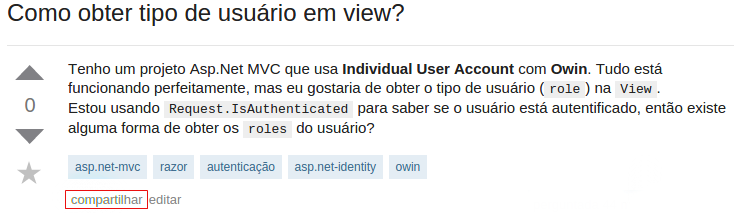
\includegraphics[scale=0.6]{./figuras/botao-compartilhar-so-pt-editado.png}
        \caption{Botão para compartilhar perguntas no site \textit{Stack Overflow em Português} destacado em bordas vermelhas no canto inferior esquerdo da imagem.}
        \label{fig:botaoCompartilharSOPT}
    \end{figure}
    
Na figura acima é possível visualizar o botão padrão existente no site \textit{Stack Overflow em Português} que serve para compartilhar perguntas deste site em redes sociais. De acordo com as análises qualitativas realizadas anteriormente, é possível que o site não consiga, por meio deste botão, fazer com que muitos usuários compartilhem perguntas em redes sociais. A partir daí surgiu a necessidade de testar tipos diferentes de botões que servissem como estratégias diferentes para tentar atrair usuários para realizar o compartilhamento de perguntas. O intuito disto era verificar os efeitos destas diferentes estratégias na quantidade de compartilhamentos de perguntas de um site \qa em redes sociais. Mais detalhes sobre tais estratégias estão na subeção Metodologia e Decisões de Projeto, mais adiante neste capítulo.

É importante constatar que uma das facetas da pesquisa em sistemas colaborativos, de acordo com Peter J. Thomas \cite{Thomas:1996:CRE:524573}, é testar alternativas de design para tais sistemas e constatar os possíveis efeitos destas alternativas na maneira com a qual os usuários lidam com eles. Portanto, é evidente que a grande motivação deste experimento foi a sua possível contribuição para a literatura da área de sistemas colaborativos.

Vale destacar que, de acordo com os relatos obtidos por meio das entrevistas com usuários de sites \qa, esperava-se que, no geral, o ato de compartilhar perguntas não seria muito comum durante a realização deste experimento.

Portanto, tendo como base tudo o que foi exposto anteriormente, a pergunta de pesquisa que guiou este experimento em questão foi a seguinte: é possível aumentar o número de compartilhamentos de perguntas oriundas de um dado site \qa em redes sociais se valendo de algum ajuste no design dos mesmos?

\section{Metodologia e Decisões de Projeto}
Foi utilizada, nesta investigação, uma abordagem empírica na forma de um estudo de caso no qual um site \qa foi desenvolvido especialmente para este experimento, tendo perguntas reais do site \textit{Stack Overflow em Português} utilizadas para fomentá-lo. Tais perguntas foram realizadas em 2014 e estavam, até o início do experimento, abertas (isto é, ainda era possível responder, votar e comentar), sem respostas e com votos positivos dos usuários.

Foi criada uma campanha com o intuito de promover o site \textit{Stack Overflow em Português}, já que na época fazia pouco mais de um ano que este site tinha sido criado. Páginas nas redes sociais \textit{Twitter} e \textit{Facebook} foram utilizadas para promover esta campanha e tentar fazer com que os usuários acessassem o site da campanha, que tinha a URL \textit{http://www.umaforcaso.pt/}.

Ao entrar no site do experimento em questão, um dado usuário se deparava com uma lista de questões com os respectivos assuntos (ver Figura~\ref{fig:printUmaForca1-2}). Era possível buscar questões informando algum assunto como parâmetro de busca. Ao clicar numa questão, era possível ler a mesma além de executar três ações: voltar para a lista de questões, responder a pergunta no \textit{Stack Overflow em Português} e compartilhar a pergunta nas redes sociais (ver Figura~\ref{fig:printUmaForca3-3}).

    \begin{figure}[H]
        \center
        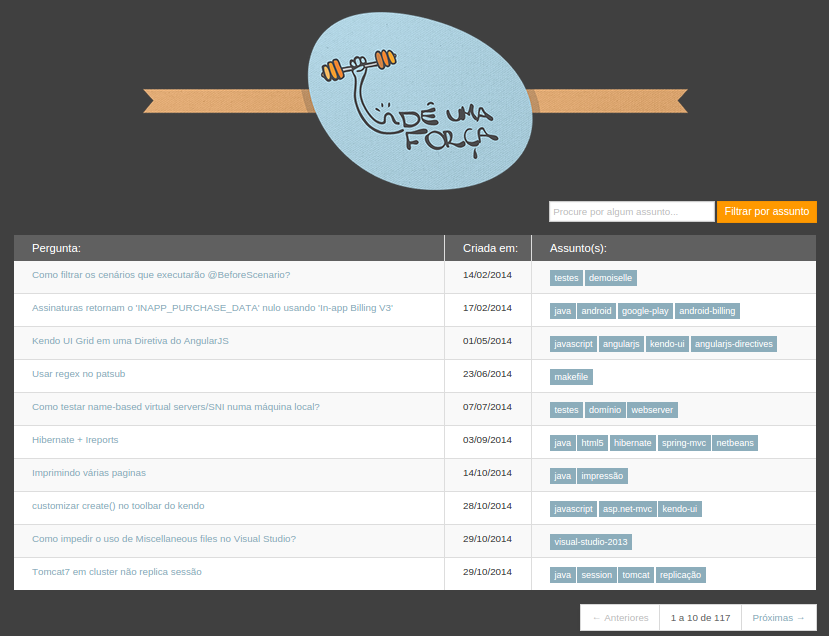
\includegraphics[scale=0.55]{./figuras/printUmaForca1-2.png}
        \caption{Página inicial do site utilizado neste experimento em questão.}
        \label{fig:printUmaForca1-2}
    \end{figure}

Ao clicar no botão de responder, um dado usuário era direcionado ao site \textit{Stack Overflow em Português} para então poder responder a pergunta por lá. O motivo da escolha deste fluxo de uso é que, desta forma, não seria necessário informar nome de usuário e senha para utilizar o site da campanha, o que poderia ser considerado como um empecílho para algumas pessoas. O design do site, no geral, foi feito de uma forma que tentasse fazer os usuários remeterem ao \textit{Stack Overflow em Português} para que eles tivessem em mente o motivo de estarem ali: ajudar a fomentar o site. Vale ressaltar que foi deixado claro, durante a campanha, que esta ajuda poderia ocorrer de duas maneiras: respondendo ou compartilhando perguntas. Os usuários sabiam que estavam de certa forma ajudando a ciência, mas não foi lhes dado nenhum outro detalhe sobre isto para tentar evitar algum tipo de viés.

Como foi explicado anteriormente, o principal motivo deste experimento em forma de uma campanha fomentadora de um site \qanospace, no caso o \textit{Stack Overflow em Português}, foi a intenção de testar estratégias diferentes para tentar atrair mais compartilhamentos de perguntas de sites deste tipo em redes sociais. Devido ao risco de algum outro elemento de design afetar o comportamento dos usuários, as estratégias testadas se diferenciavam entre si apenas na mensagem exibida no botão de compartilhar. Como explicação para isto, estes usuários disseram que os ganhos sociais relacionados a esta prática não estão claros e se ninguém faz isto é porque as pessoas talvez não gostem muito de receber conteúdos assim nas suas redes sociais. 

    \begin{figure}[H]
        \center
        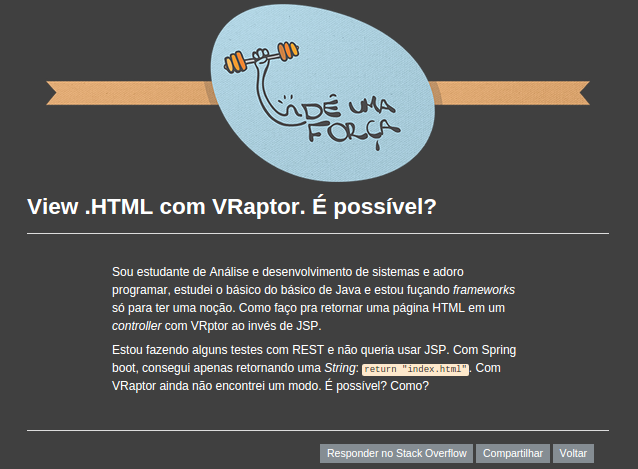
\includegraphics[scale=0.7]{./figuras/printUmaForca3-3.png}
        \caption{Uma pergunta visualizada no site utilizado neste experimento em questão.}
        \label{fig:printUmaForca3-3}
    \end{figure}
    
Ao clicar no botão de compartilhar, os participantes tinham as opções de compartilhar a pergunta em questão nas redes sociais \textit{Google+}, \textit{Facebook} e \textit{Twitter}, tal qual acontece no cenário real (ou seja, no site \textit{Stack Overflow em Português}). Os participantes do experimento foram divididos em três grupos distintos. Cada grupo só conseguia visualizar um único respectivo tipo de mensagem no botão de compartilhar. A primeira mensagem, denominada mensagem 1, era a mesma que existe no próprio site \textit{Stack Overflow em Português} (ver Figura~\ref{fig:printUmaForca4}), as outras duas foram elaboradas de acordo com as investigações qualitativas realizadas anteriormente e foram tentativas de enaltecer aspectos positivos do ato de compartilhar perguntas em redes sociais, de acordo com os relatos obtidos nas investigações qualitativas deste trabalho. 

    \begin{figure}[H]
        \center
        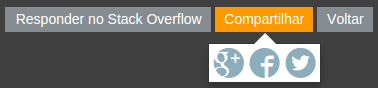
\includegraphics[scale=0.7]{./figuras/printUmaForca4.png}
        \caption{Mensagem padrão utilizada para atrair compartilhamentos.}
        \label{fig:printUmaForca4}
    \end{figure}

A segunda mensagem, denominada mensagem 2 (ver Figura\ref{fig:printUmaForca5}), se caracteriza pelo seguinte texto: \textit{"Algumas pessoas costumam compartilhar para ajudar. Compartilhe!"}. A motivação para a escolha desta mensagem é o fato de que usuários de sites \qa relataram, na primeira investigação qualitativa, que acreditavam que quase ninguém costuma compartilhar perguntas destes sites em redes sociais e usaram esta constatação como uma das justificativas para não se comportar de tal maneira. Os pesquisadores, então, elaboraram esta mensagem como forma de convencer os usuários de que existem pessoas que compreendem os ganhos sociais relacionados a esta prática e, portanto, este comportamento não é tão incomum.

    \begin{figure}[H]
        \center
        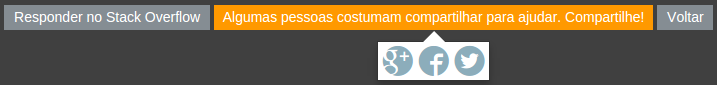
\includegraphics[scale=0.6]{./figuras/printUmaForca5.png}
        \caption{Segunda mensagem utilizada para atrair compartilhamentos.}
        \label{fig:printUmaForca5}
    \end{figure}

A terceira e última mensagem, denominada mensagem 3 (ver Figura\ref{fig:printUmaForca6}), é a seguinte: \textit{"Algum amigo seu pode saber a resposta. Compartilhe!"}. Nas duas investigações qualitativas, os usuários relataram que utilizam redes sociais para reforçar ou criar novos laços sociais. Interagir com amigos e com outras pessoas foi uma das justificativas dadas tanto por usuários que costumam compartilhar perguntas de outros nas redes sociais quanto por aqueles que não costumam agir assim. Utilizando o termo \textit{amigo}, os pesquisadores tentaram convencer os participantes de que existe um elo claro entre o site \qa em questão e as redes sociais. Esta mensagem foi uma tentativa de fazer o participante pensar em algum amigo que poderia de fato saber a resposta e o qual valesse a pena, em termos de capital social, tentar interagir desta forma em alguma rede social.

    \begin{figure}[H]
        \center
        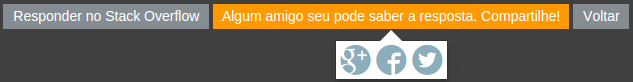
\includegraphics[scale=0.7]{./figuras/printUmaForca6.png}
        \caption{Terceira mensagem utilizada para atrair compartilhamentos.}
        \label{fig:printUmaForca6}
    \end{figure}

Evidentemente, outras mensagens poderiam ser elaboradas para serem utilizadas no experimento. Entretanto, quanto maior fosse a quantidade de grupos de usuários (um grupo para cada mensagem) maior deveria ser a quantidade total de usuários utilizando o site do experimento. Por este motivo, para este escopo, optou-se por utilizar apenas três mensagens no botão de compartilhar perguntas em redes sociais. 

Visando atrair mais participantes para o experimento, foi feita uma campanha de divulgação paga na rede social \textit{Facebook}. Tal campanha durou apenas uma semana devido a restrições orçamentárias da pesquisa. Alguns dados dos relatórios gerados sobre os acessos ao site desta campanha em questão encontram-se nos apêndices deste documento.

O site para realizar o experimento foi desenvolvido com o auxílio das seguintes tecnologias:
    \begin{itemize}
        \item \textit{Play Framework} \cite{hunt2014play} - \textit{framework} para desenvolvimento de aplicações \textit{web};
        \item \textit{Scala} \cite{odersky2008programming} - linguagem de programação de propósito geral que foi utilizada para construir o \textit{back-end} da aplicação;;
        \item \textit{HTML} \cite{pilgrim2010html5} - linguagem de marcação utilizada para construir páginas na \textit{web};
        \item \textit{JavaScript} \cite{flanagan2006javascript} e \textit{CoffeeScript} \cite{maccaw2012little} - linguagens de programação amplamente difundidas e utilizadas na construção de páginas dinâmicas na \textit{web};
        \item \textit{PostgreSQL} \cite{obe2014postgresql} - sistema gerenciador de banco de dados objeto-relacional;
        \item \textit{Git} \cite{loeliger2012version} - sistema de controle de versão;
        \item \textit{Heroku} \cite{middleton2013heroku} - plataforma de serviço em nuvem utilizada para hospedar aplicações \textit{web} nas nuvens, utilizando a tecnologia de computação nas nuvens, eliminando a necessidade do dono da aplicação contratar um servidor físico diretamente.
    \end{itemize}

\section{Dados Coletados e Análise dos Resultados}
O site da campanha fomentadora do \textit{Stack Overflow em Português} ficou no ar durante exatos 30 dias. Durante este tempo, foram coletados dados relativos à quantidade de: usuários, compartilhamentos e visualizações de perguntas e do botão de compartilhar. Além destes dados, também foram salvos no banco de dados informações sobre quem compartilhou qual pergunta e qual era a mensagem exibida no botão de compartilhar no momento de cada compartilhamento realizado. Por fim, também foi possível extrair do banco de dados informações detalhadas sobre perguntas visualizadas que não foram compartilhadas: quem era o usuário em questão, qual era a pergunta e qual era a mensagem do botão de compartilhar naquele momento. Vale ressaltar que tais dados foram estatisticamente analisados utilizando a linguagem de programação \textit{R} \cite{chapman2015overview}.

A grande contribuição deste experimento, como foi dito anteriormente, foi o fato de que alternativas de design (mensagens diferentes no botão de compartilhar perguntas de um site \qa em redes sociais) foram testadas para verificar o efeito das mesmas na quantidade de compartilhamentos realizados. Portanto, havia a necessidade de categorizar os compartilhamentos realizados durante o experimento em três grupos: cada grupo deveria estar relacionado com uma das três mensagens utilizadas neste experimento e explicadas na seção anterior deste capítulo.

78 participantes distintos visualizaram as mensagens do botão de compartilhar (isto é, visualizaram perguntas no site do experimento). Vale ressaltar  que quase todos estes usuários visualizaram mais do que uma única pergunta. Destes usuários, 25 viram apenas a mensagem 1, 23 viram apenas a mensagem 2 e 30 viram apenas a mensagem 3. 

Como era esperado de acordo com os relatos obtidos nas investigações qualitativas, o número de pessoas que compartilharam perguntas do site do experimento em redes sociais não foi alto: apenas 15,39\% dos usuários que leram as mensagens no botão de compartilhar realizaram compartilhamento em redes sociais. Destes, nenhum viu a mensagem 1. Ou seja: nenhum usuário que se deparou com a mensagem "\textit{Compartilhar}" compartilhou alguma pergunta (ver Figura~\ref{fig:piechart1}).

    \begin{figure}[H]
        \center
        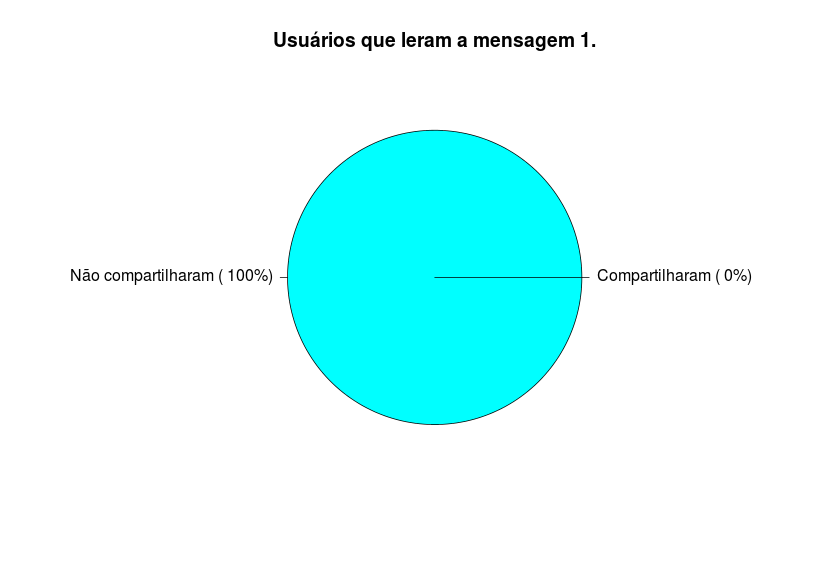
\includegraphics[scale=0.4]{./figuras/piechart-virammsg1-2.png}
        \caption{Gráfico de setores representando a proporção entre os usuários que compartilharam perguntas e os que não compartilharam, dentre os que viram a mensagem 1.}
        \label{fig:piechart1}
    \end{figure}
    
Apenas 3,85\% dos participantes que visualizaram as mensagens compartilharam perguntas enquanto estavam vendo a mensagem 2 ("\textit{Algumas pessoas costumam compartilhar para ajudar. Compartilhe!}") no botão de compartilhar. Dentre os usuários que se depararam com esta mensagem, 13,0\% compartilharam alguma pergunta em alguma rede social. Uma representação desta proporção pode ser visualizada na Figura~\ref{fig:piechart2}.

11,54\% dos participantes que visualizaram as mensagens compartilharam perguntas enquanto estavam vendo a mensagem 3 (\textit{"Algum amigo seu pode saber a resposta. Compartilhe!"}) no botão de compartilhar. Dentre os usuários que se depararam com esta mensagem, 30,0\% compartilharam alguma pergunta em alguma rede social. Uma representação desta proporção pode ser visualizada na Figura~\ref{fig:piechart3}.

É possível constatar, portanto, que existe uma proporção maior de usuários que compartilharam perguntas em alguma rede social enquanto estavam visualizando a mensagem 3. A Figura~\ref{fig:barchart1}  e a Figura~\ref{fig:piechart4} podem ser utilizadas como auxílio nesta ilustração.

    \begin{figure}[H]
        \center
        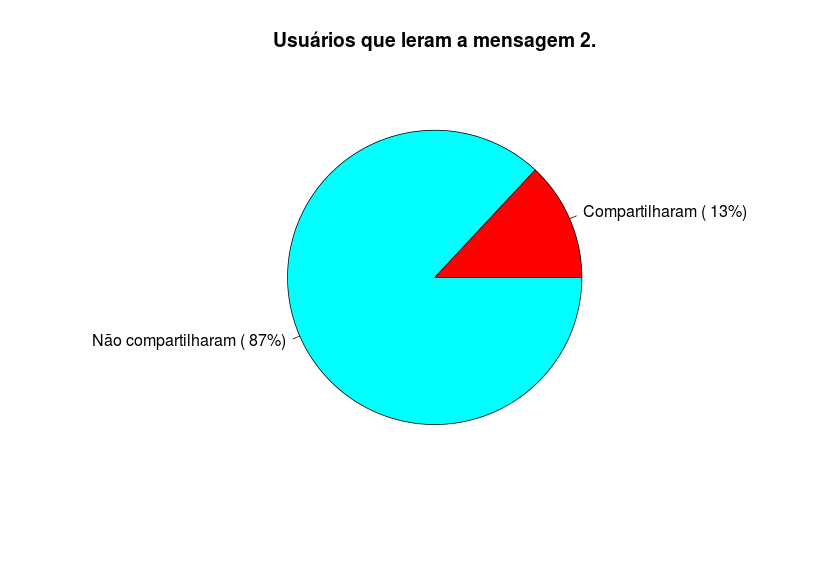
\includegraphics[scale=0.4]{./figuras/piechart-virammsg2-2.png}
        \caption{Gráfico de setores representando a proporção entre os usuários que compartilharam perguntas e os que não compartilharam, dentre os que viram a mensagem 2.}
        \label{fig:piechart2}
    \end{figure}
    
    \begin{figure}[H]
        \center
        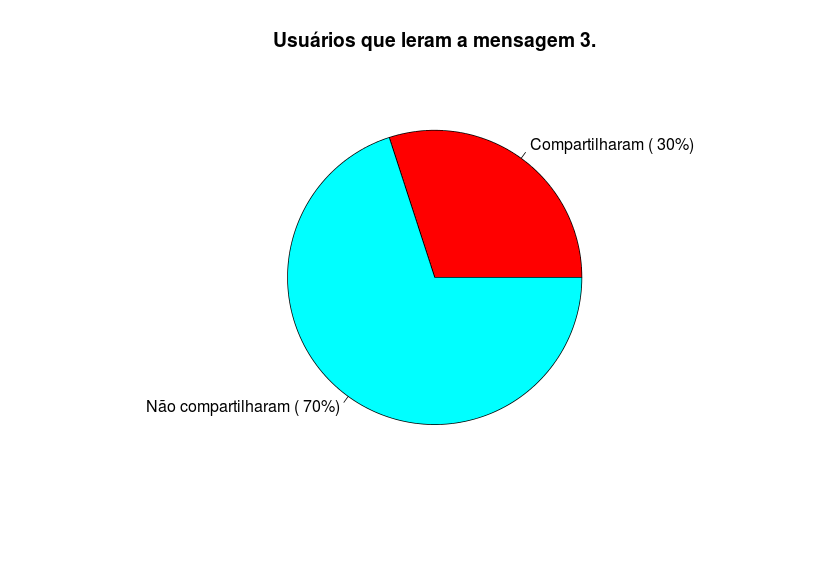
\includegraphics[scale=0.4]{./figuras/piechart-virammsg3-2.png}
        \caption{Gráfico de setores representando a proporção entre os usuários que compartilharam perguntas e os que não compartilharam, dentre os que viram a mensagem 3.}
        \label{fig:piechart3}
    \end{figure}

Em termos estatísticos, a principal intenção dos pesquisadores neste experimento era observar a relação entre o tipo de mensagem exibida no botão de compartilhar e o fato de uma pergunta ter sido compartilhada ou não. Note que foram criadas duas variáveis categórias para classificar os usuários: uma diz respeito ao tipo de mensagem que os usuários visualizaram e a outra diz respeito ao fato de um dado usuário ter ou não compartilhado alguma pergunta em alguma rede social. A primeira variável poderia assumir três valores distintos: 1, 2, ou 3, já que foram testadas três alternativas de design. A segunda variável, por sua vez, poderia assumir apenas os valores lógicos verdadeiro ou falso.

De acordo com Field et al. \cite{field2012discovering}, quando existe a necessidade de verificar se duas variáveis categóricas estão ou não relacionadas, geralmente se utiliza o teste estatístico qui-quadrado de Pearson. Entretanto, quando a quantidade de dados coletados não é grande o suficiente, é preferível utilizar o teste exato de Fisher. Note que poucos usuários, no geral, compartilharam perguntas e, inclusive, nenhum usuário compartilhou quando se deparou com a mensagem 1. Por isto escolhemos o último teste estatístico citado para procurar indícios estatísticos sobre a relação entre o tipo de mensagem no botão de compartilhar e a quantidade de compartilhamentos.

    \begin{figure}[H]
        \center
        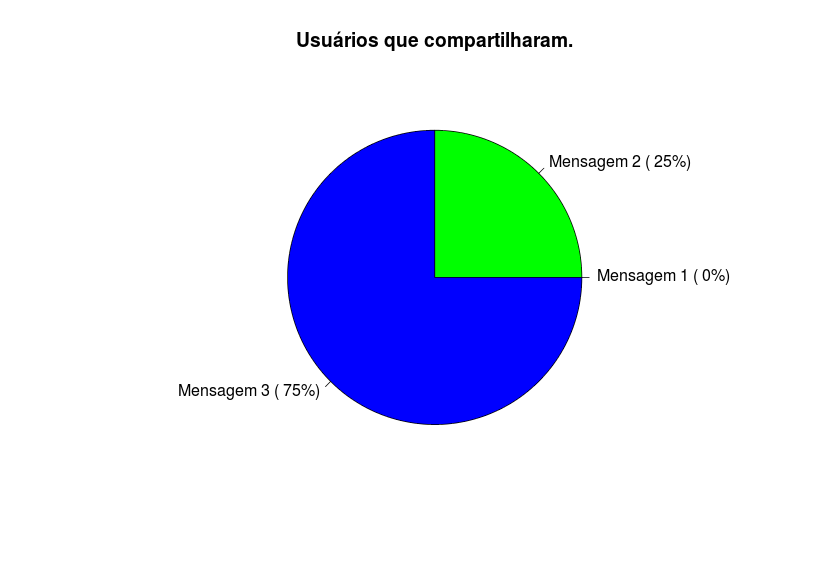
\includegraphics[scale=0.4]{./figuras/piechart-compartilharam-2.png}
        \caption{Gráfico de setores representando as mensagens visualizadas pelos usuários que compartilharam perguntas.}
        \label{fig:piechart4}
    \end{figure}
    
    Para iniciar a análise estatística, primeiro foi construída uma tabela de contigência para contar quantos usuários faziam parte de cada categoria (ver a Tabela 5.1). Uma representação desta tabela foi, dentro de um \textit{script} feito em \textit{R}, passada como parâmetro para o teste estatístico em questão. O teste exato de Fisher foi utilizado para aceitar ou refutar as seguintes hipóteses:
    \begin{itemize}
        \item \textbf{Hipótese nula}: não existe qualquer relação entre a mensagem exibida no botão de compartilhar e a quantidade de compartilhamentos realizados;
        \item \textbf{Hipótese alternativa}: existe alguma relação entre a mensagem exibida no botão de compartilhar e a quantidade de compartilhamentos realizados.
    \end{itemize}
    
    \begin{figure}[H]
        \center
        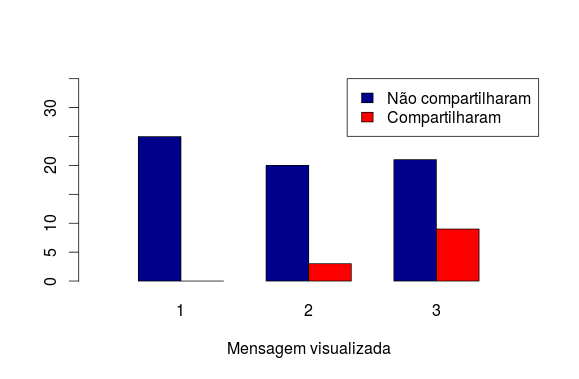
\includegraphics[scale=0.7]{./figuras/barchart-compartilhamentos.png}
        \caption{Gráfico de barras mostrando as comparações entre as quantidades de usuários que compartilharam e que não o fizeram, para cada uma das três alternativas de design testadas.}
        \label{fig:barchart1}
    \end{figure}
    
    Para executar o teste exato de Fisher por meio de um \textit{script} em \textit{R}, foi necessário utilizar uma função desenvolvida por Marc Schwartz chamada \textit{CrossTable} \cite{crosstable}. Dentre vários resultados, além de um p-valor, tal função retornou para cada contagem presente na tabela de contigência: o valor esperado se não houvesse qualquer relação entre as variáveis analisadas e o valor dos resíduos padrão tal qual a fórmula descrita por Field et al. \cite{field2012discovering}. 

% Please add the following required packages to your document preamble:
% \usepackage{multirow}
% \usepackage[table,xcdraw]{xcolor}
% If you use beamer only pass "xcolor=table" option, i.e. \documentclass[xcolor=table]{beamer}
\begin{table}[h]
\centering
\label{tab:tab1}
\begin{tabular}{ccc}
\hline
\cellcolor[HTML]{C0C0C0}{\color[HTML]{333333} }                                       & \multicolumn{2}{l}{\cellcolor[HTML]{C0C0C0}Compartilhou?} \\ \cline{2-3} 
\multirow{-2}{*}{\cellcolor[HTML]{C0C0C0}{\color[HTML]{333333} Mensagem visualizada}} & Não                          & Sim                        \\ \hline
1                                                                                     & \cellcolor[HTML]{EFEFEF}25   & \cellcolor[HTML]{EFEFEF}0  \\ \hline
2                                                                                     & \cellcolor[HTML]{EFEFEF}20   & \cellcolor[HTML]{EFEFEF}3  \\ \hline
3                                                                                     & \cellcolor[HTML]{EFEFEF}21   & \cellcolor[HTML]{EFEFEF}9  \\ \hline
\end{tabular}
\caption{Tabela de contigência construída com os dados coletados durante este experimento para a realização do teste exato de Fisher.}
\end{table}

A execução to teste exato de Fisher retornou um p-valor igual a 0,004928519. Ou seja, a chance da configuração dos valores coletados ser resultante do acaso e não da influência exercida por algum fator estudado é menor do que 0,5\%. Como este valor é menor do que 0,05, então a hipótese nula foi rejeitada com um nível de significância igual a 0,05. Ou seja: a chance de a hipótese nula estar errada e a hipótese alternativa estar certa é de 95\%. Portanto, com 95\% de certeza, é possível afirmar que existe alguma relação entre a mensagem exibida no botão decompartilhar e a quantidade de compartilhamentos realizados.

Na Tabela 5.2, é possível visualizar uma tabela de contigência construída com demais os resultados do teste estatístico executado.

% Please add the following required packages to your document preamble:
% \usepackage{multirow}
% \usepackage[table,xcdraw]{xcolor}
% If you use beamer only pass "xcolor=table" option, i.e. \documentclass[xcolor=table]{beamer}
\begin{table}[h]
\centering
\label{tab:tab2}
\begin{tabular}{|c|l|c|c|}
\hline
\multicolumn{2}{|c|}{}                                       & \multicolumn{2}{c|}{Compartilhou?}                              \\ \cline{3-4} 
\multicolumn{2}{|c|}{\multirow{-2}{*}{Mensagem visualizada}} & Não                            & Sim                            \\ \hline
\multicolumn{2}{|c|}{}                                       & \cellcolor[HTML]{67FD9A}25     & \cellcolor[HTML]{67FD9A}0      \\
\multicolumn{2}{|c|}{}                                       & \cellcolor[HTML]{FD6864}21,154 & \cellcolor[HTML]{FD6864}3,846  \\
\multicolumn{2}{|c|}{\multirow{-3}{*}{1}}                    & \cellcolor[HTML]{C0C0C0}0,836  & \cellcolor[HTML]{C0C0C0}-1,961 \\ \hline
\multicolumn{2}{|c|}{}                                       & \cellcolor[HTML]{67FD9A}20     & \cellcolor[HTML]{67FD9A}3      \\
\multicolumn{2}{|c|}{}                                       & \cellcolor[HTML]{FD6864}19,462 & \cellcolor[HTML]{FD6864}3,538  \\
\multicolumn{2}{|c|}{\multirow{-3}{*}{2}}                    & \cellcolor[HTML]{C0C0C0}0,122  & \cellcolor[HTML]{C0C0C0}-0,286 \\ \hline
\multicolumn{2}{|c|}{}                                       & \cellcolor[HTML]{67FD9A}21     & \cellcolor[HTML]{67FD9A}9      \\
\multicolumn{2}{|c|}{}                                       & \cellcolor[HTML]{FD6864}25,385 & \cellcolor[HTML]{FD6864}4,615  \\
\multicolumn{2}{|c|}{\multirow{-3}{*}{3}}                    & \cellcolor[HTML]{C0C0C0}-0,870 & \cellcolor[HTML]{C0C0C0}2,041  \\ \hline
\end{tabular}
\caption{Tabela de contigência resultante da análise estatística realizada. Em tom de verde encontram-se os valores coletados durante o experimento. Em tom de vermelho encontram-se os valores esperados, calculados pelo teste estatístico realizado, caso não houvesse relação entre as variáveis estudadas. Por fim, em tom de cinza, encontram-se os resíduos padrão que são os erros entre o que o teste esperava acontecer (valores esperados) e o que realmente aconteceu (valores coletados).}
\end{table}

Merecem destaque dois cenários: a quantidade de pessoas que compartilharam perguntas enquanto estavam visualizando a mensagem 3 e a quantidade de pessoas que não compartilharam perguntas enquanto estavam visualizando a mensagem 1. 

Para o primeiro cenário supracitado, observe que o valor coletado foi 9, o valor esperado era 4,615 e o resíduo padrão calculado é igual a 2,041. É possível perceber que mais usuários visualizaram a mensagem 3 e compartilharam perguntas do que se esperava. Como o valor do resíduo padrão é positivo e maior do que 1,96, então, ainda de acordo com Field et al. \cite{field2012discovering}, a mensagem 3 exerceu uma influência significativa e positiva na quantidade de usuários que compartilharam perguntas.  

Para o segundo cenário citado anteriormente, observe que o valor coletado foi 0, o valor esperado era 3,846 e o resíduo padrão calculado é igual a -1,961. É possível perceber que a quantidade de usuários que visualizaram a mensagem 1 e não compartilharam nenhuma pergunta nas redes sociais foi menor do que o que se esperava. Como o valor do resíduo padrão é negativo e um pouco menor do que -1,96, é possível afirmar que a mensagem 1 exerceu certa influência significativa e negativa na quantidade de usuários que compartilharam perguntas. Para todos os outros cenários, pode-se afirmar que os dados coletados não foram significativamente diferentes do esperado. 

Ainda é possível afirmar que a mensagem 2 exerceu uma influência positiva maior no número de compartilhamentos do que a mensagem 1, embora menor do que a influência exercida pela mensagem 3.

Por fim, é importante destacar que apenas uma única pergunta, dentre as que foram compartilhadas em redes sociais, foi respondida. O que pode ser um indicativo de que compartilhar perguntas oriundas de sites \qa em redes sociais pode não funcionar muito bem como estratégia fomentadora de conteúdo para tais sites. Entretanto, fica evidente que seria necessário mais dados coletados para que algum teste estatístico pudesse ser realizado e, desta forma, pudéssemos afirmar algo com mais relevância estatística sobre a utilidade ou não do compartilhamento de perguntas neste âmbito.

\chapter{Conclusões Finais}

\section{Contribuições}

\section{Limitações e Trabalhos Futuros}  

%%%%%%%%%%%%%%%%%%%%%%%%%%%%%%%%%%%%%%%%%%%%%%%%%%%%%%%%%%%%%%%%%%%%%%%%%%%%%%%%
%% BIbliografia
%% Coloque suas referencias no arquivo ref.bib e descomente as proximas duas linhas

\bibliographystyle{plain} % estilo de bibliografia   plain,unsrt,alpha,abbrv.
\bibliography{ref} % arquivos com as entradas bib.

%%%%%%%%%%%%%%%%%%%%%%%%%%%%%%%%%%%%%%%%%%%%%%%%%%%%%%%%%%%%%%%%%%%%%%%%%%%%%%%%
%% Apendice
% Caso seja necessario algum apendice, descomente a proxima linha.

\appendix
\chapter{Meu primeiro ap�ndice}

\chapter{Meu segundo ap�ndice}

%%%%%%%%%%%%%%%%%%%%%%%%%%%%%%%%%%%%%%%%%%%%%%%%%%%%%%%%%%%%%%%%%%%%%%%%%%%%%%%%

\end{document}